% !TEX root = mth727_lecture_notes.tex


\chapter{Review: CW Complexes}
\chaptermark{Review: CW Complexes}
\thispagestyle{firststyle}

\begin{definition}
Let $X$ be a space and let $f\colon S^{n-1} \to X$ be a continuous function. 
We say that a space $Y$ is obtained by \emph{attaching an $n$-cell}
to $X$ if $Y = X \sqcup D^{n}/{\sim}$
where $\sim$ is the equivalence relation given by $x\sim f(x)$ for all $x\in S^{n-1}\subseteq D^{n}$. 
We write $Y = X \cup_{f} e^{n}$. 

\begin{tikzpicture}
\node[anchor=south west,inner sep=0] at (0,0) 
{{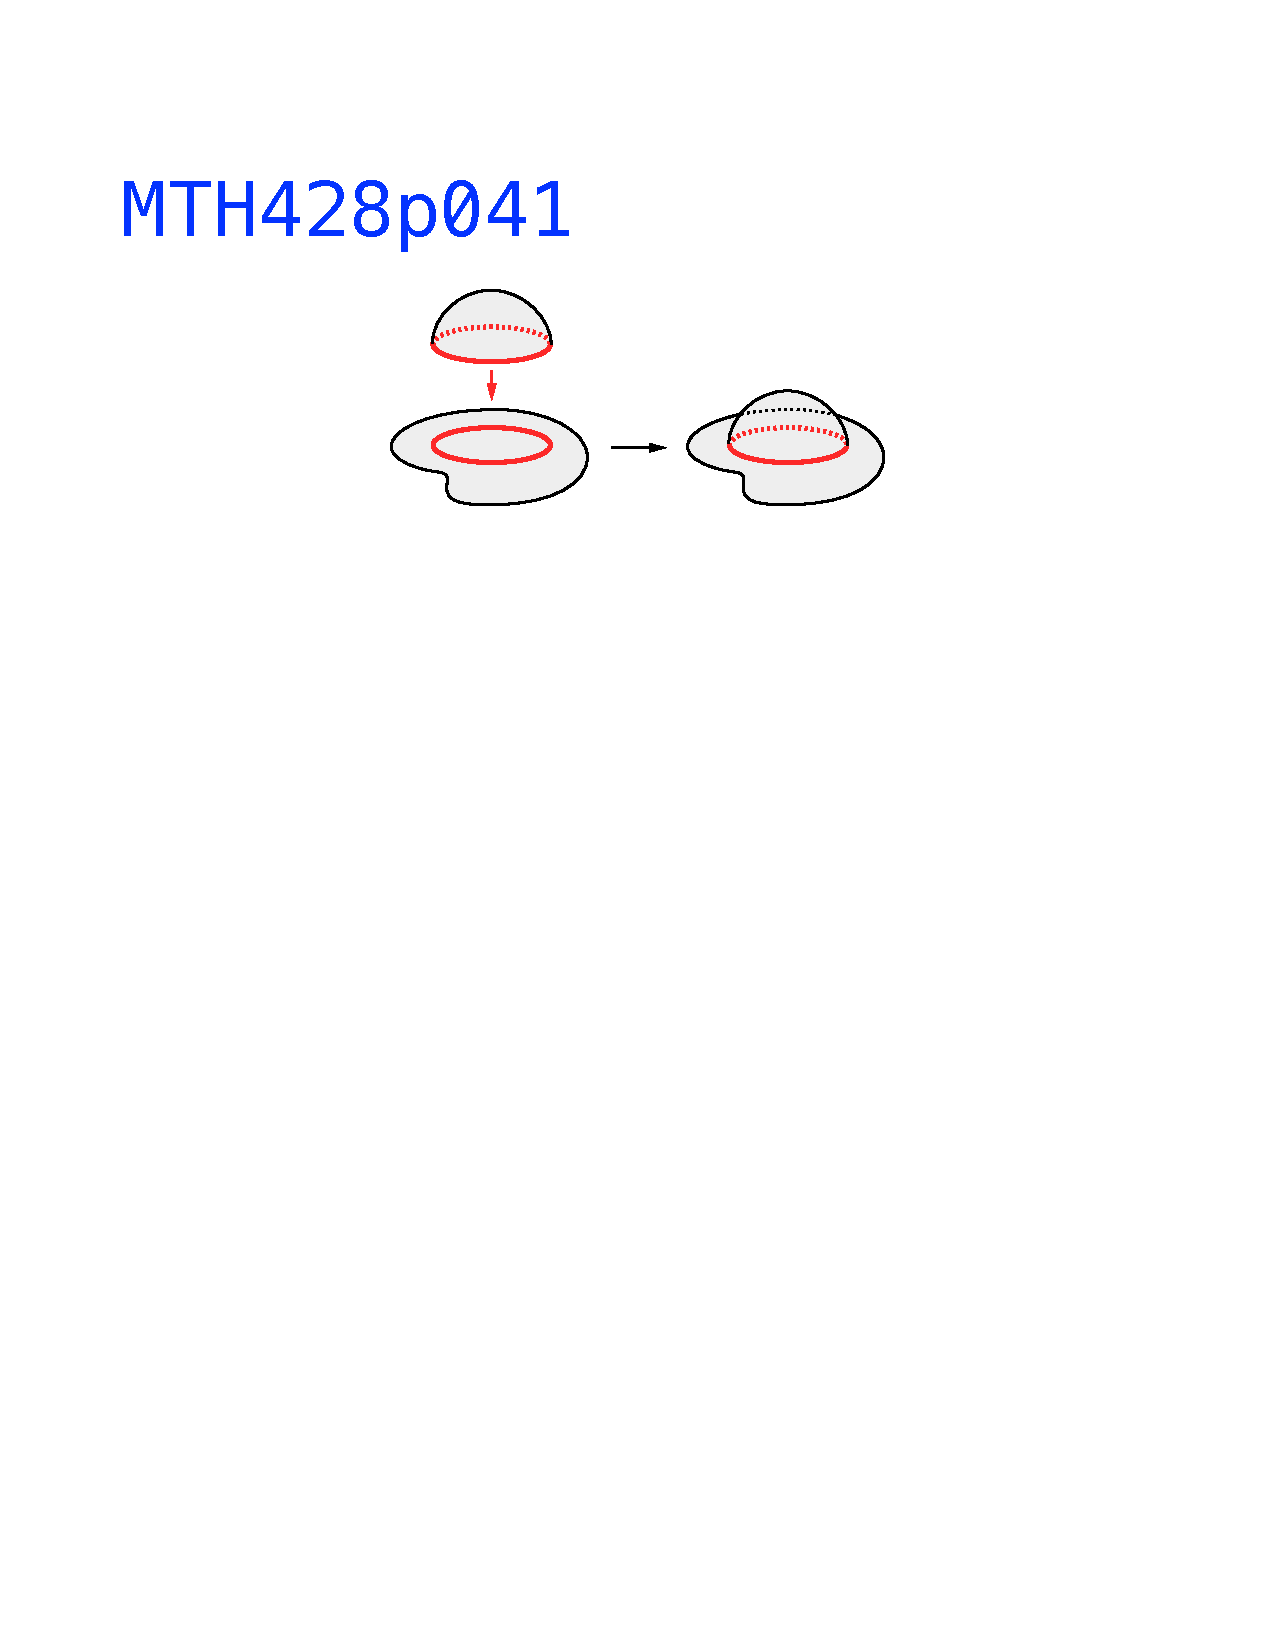
\includegraphics[width=\textwidth, trim=0mm 192mm 0mm 48mm, clip]{pictures/MTH428p041.pdf}}};

%%% COORDINATE GRID
%\draw[step=0.5, help lines] (0,0) to[grid with coordinates] (15,9);
%%% 

\node[anchor=  base]  at (6.7 , 1.6){\color{red} \small  $f$};
\end{tikzpicture}

\end{definition}


\begin{nn}
\label{CW TERMINOLOGY NN}
%---EBLANK  #  {\bf Some terminology.}
%---BBLANK  #
Some terminology:

\benu
\item[\textbullet] The map $f\colon S^{n-1} \to X$ is called the \emph{attaching map} of the cell $e^{n}$. 
\item[\textbullet]  The map $\bar{f} \colon D^{n} \to X \sqcup D^{n} \to X\cup_{f} e^{n}$ is called 
the \emph{characteristic map} of the cell $e^{n}$. 
\item[\textbullet] The subspace $e^{n} = \bar{f}(D^{n}\ssmin S^{n-1}) \subseteq X\cup_{f}e^{n}$ is called 
the \emph{open cell}. 
\item[\textbullet] The subspace $\xov{e}^{n} = \bar{f}(D^{n}) \subseteq X\cup_{f}e^{n}$ is called 
the \emph{closed cell}. 
\eenu
\end{nn}


\begin{proposition}
\label{CELLSLIDE PROP}
If $f, g\colon S^{n-1}\to X$ are maps such that $f\simeq g$ then $X\cup_{f} e^{n} \simeq X\cup_{g} e^{n}$. 
\end{proposition}


\begin{definition}
\label{RELCW DEF}
Let $X$ be topological space and let $A\subseteq X$. The pair $(X, A)$ is 
a \emph{relative CW complex} if $X = \bigcup_{n=-1}^{\infty} X^{(n)}$
where 
\benu
\item[1)]
$X^{(-1)} = A$;
\item[2)] for $n\geq 0$ the space $X^{(n)}$ is obtained by attaching $n$-cells to $X^{(n-1)}$;
\item[3)] the topology on $X$ is defined so that a set $U\subseteq X$ is open if and only if
$U\cap X^{(n)}$ is open in $X^{(n)}$ for all $n$. 
\eenu
\end{definition}


\begin{note}
If $(X, A)$ is a relative CW complex then the space $X^{(n)}$ is called the \emph{$n$-skeleton}
of $X$. 
\end{note}


\begin{note}
\label{CW CONT FUNCTIONS NOTE}
By part 3) of Definition \ref{RELCW DEF} if $(X, A)$ is a relative CW complex then a function 
$f\colon X\to Z$ is continuous if and only if $f|_{X^{(n)}}\colon X^{(n)} \to Z$ is continuous for all $n\geq -1$. 
\end{note}


\begin{note}
Assume that $(X, A)$ is a relative CW complex and that we are given a map $g\colon A\to Z$. 
In such situation, we will often want to construct a map $\xov{g} \colon X \to Z$ 
such that $\xov{g}|A = g$. Usually, this construction will proceed inductively 
with respect to the skeleta of $X$. We will assume that we have already constructed a map 
$\xov{g}_{n-1}\colon X^{(n-1)} \to Z$ such that $\xov{g}_{n-1}|_{A} = g$, and we 
will attempt to extend $\xov{g}_{n-1}$ to $\xov{g}_{n}\colon X^{(n)} \to Z$.   
The space $X^{(n)}$ is the quotient space of 
$X^{(n-1)} \sqcup \bigsqcup_{i} D^{n}$ with the equivalence relation defined by the attaching 
maps of $n$-cells. Therefore, to define $\xov{g}_{n}$ it will suffice, for each $n$-cell 
$e^{n}$ with the attaching map $f\colon S^{n-1}\to Z$, to give a map $\varphi\colon D^{n}\to Z$ 
such that $\varphi|_{S^{n-1}} = \xov{g}_{n-1}f$.  

Once we have maps $\xov{g}_{n}$ for all $n$, we can define $\xov{g}\colon X \to Z$
by setting $\xov{g}|_{X^{(n)}} = \xov{g}_{n}$. The map $\xov{g}$ is continuous 
by (\ref{CW CONT FUNCTIONS NOTE}). 
\end{note}




\begin{definition}
A \emph{CW complex}  is a space $X$ such that $(X, \varnothing)$
is a relative CW complex.  
\end{definition}


\begin{definition}
1) A CW complex $X$ is \emph{finite} if it consists of finitely many cells. 

2) A CW complex $X$ is \emph{finite dimensional} if $X= X^{(n)}$ for some $n$. 

3) The \emph{dimension} of a CW complex $X$ is defined by 
$$
\dim X =
\begin{cases}
\min\{n \ | \  X = X^{(n)} \} & \text{ if $X$ is finite dimensional} \\
\infty  & \text{otherwise}
\end{cases}
$$
\end{definition}

\begin{definition}
Let $X, Y$ be relative CW complexes. A map $f\colon X \to Y$ is \emph{cellular} if $f(X^{(n)}) \subseteq Y^{(n)}$
for all $n\geq 0$. 
\end{definition}


\begin{CELLAPPROXTHM}
\label{CELLAPPROX THM}
Let $X, Y$ be relative CW complexes. For any map $f\colon X \to Y$ there exists a cellular map 
$g\colon X \to Y$ such that $f\simeq g$. Moreover, if $A\subseteq X$ is a subcomplex and 
$f|_{A}\colon A \to Y$ is a cellular map then $g$ can be selected so that   
$f|_{A} = g|_{A}$ and $f\simeq g \ (\rel A)$.
\end{CELLAPPROXTHM}


\begin{corollary}
\label{SMSNCONTRACT COR}
If $n> m$ then every map $f\colon S^{m} \to S^{n}$ is homotopic to a constant map. 
\end{corollary}

\begin{proof}
Consider $S^{n}$ with the structure of a CW complex with one $0$-cell and 
one $n$-cell. By Theorem \ref{CELLAPPROX THM} any map $f\colon S^{m}\to S^{n}$
is homotopic to a cellular map. Since the $m$-skeleton of $S^{n}$ consists of 
a single point, such a cellular map is constant.
\end{proof}


\begin{definition}
Let $X$ be a topological space, and let $A\subseteq X$. The pair $(X, A)$ has the 
\emph{homotopy extension property} if any map 
$$h\colon X\times \{0\} \cup A\times [0, 1] \to Y$$
can be extended to a map $\bar{h}\colon X \times [0, 1] \to Y$.  
\end{definition}


\begin{theorem}
\label{HEP REL CW THM}
Any relative CW complex $(X, A)$ has the homotopy extension property. 
\end{theorem}

\begin{proposition}
\label{CONTR QUOTIENT WITH HEP PROP}
If $(X, A)$ has the homotopy extension property and $A$ is a contractible space, then the quotient map  $q\colon X \to X/A$ is a homotopy equivalence. 
\end{proposition}


\begin{INDUCTIVEHOMOTLEMMA}
\label{INDUCTIVEHOMOT LEMMA}
Let $(X, A)$ be a relative CW complex and let $A = X_{-1} \subseteq X_{0}\subseteq X_{1} \subseteq \dots  \subseteq X$
be subcomplexes of $X$ such that $\bigcup_{n} X_{n} = X$. Assume that for $n\geq -1$ we have 
maps $f_{n}\colon X \to Y$ such that 
\benu
\item $f_{n}|_{X_{n-1}} = f_{n-1}|_{X_{n-1}}$ for all $n \geq 0$
\item $f_{n}\simeq f_{n-1} \ (\rel X_{n-1})$ for all $n\geq 0$
\eenu
Let $g\colon X \to Y$ be given by $g(x) = f_{n}(x)$ if $x\in X_{n}$. 
Then $g$ is a continuous function and $f_{-1}\simeq g \  (\rel A)$.
\end{INDUCTIVEHOMOTLEMMA}

\begin{example}
Take
$$S^{n} = \left\{(x_{1},\dots, x_{n+1})\in \R^{n+1} \ | \ \sum_{i=1}^{n+1} x_{i}^{2} = 1\right\}$$
Denote also $S^{-1} = \varnothing$.
For each $n$ we have an embedding $j\colon S^{n} \hra S^{n+1}$ given by 
$j(x_{1}, \dots, x_{n+1}) = (x_{1}, \dots, x_{n+1}, 0)$. 
Define $S^{\infty} = \bigcup_{n} S^{n}$. A set $U\subseteq S^{\infty}$ is open if for each 
$n \geq 0$ the set $U\cap S^{n}$ is open in $S^{n}$. 

The space $S^{\infty}$ has a CW complex structure where $S^{n}$ is the $n$-skeleton 
of $S^{\infty}$. 
\end{example}


\begin{proposition}
\label{SINFTY CONTRACTIBLE PROP}
$S^{\infty}$ is a contractible space. 
\end{proposition}

\begin{proof}
Let $x_{0}\in S^{0}\subseteq S^{\infty}$. We can assume that $S^{\infty}$ has a 
CW complex structure such that $x_{0}$ is a $0$-cell. 
By Lemma \ref{INDUCTIVEHOMOT LEMMA} it will suffice to construct functions 
$f_{n}\colon S^{\infty} \to S^{\infty}$ for $n\geq 0$ such that 
\benu
\item $f_{-1} = \id_{S^{\infty}}$
\item $f_{n}|_{S^{n}} = x_{0}$ for all $n\geq 0$
\item $f_{n}\simeq f_{n-1} \ (\rel S^{n-1})$ for all $n\geq 0$
\eenu
We will construct functions $f_{n}$ by induction with respect to $n$. Assume that we 
already have a function $f_{n}$ satisfying the above properties. This, in particular, 
means that $f_{n}|_{S^{n}} = x_{0}$. We want to get a function $f_{n+1}$ such that 
$f_{n+1}|_{S^{n+1}} = x_{0}$ and $f_{n}\simeq f_{n+1} \ (\rel S^{n})$.
By Theorem \ref{CELLAPPROX THM}, the function $f_{n}$ is homotopic $(\rel S^{n})$ 
to a cellular function $g\colon S^{\infty} \to S^{\infty}$. The function 
$g$ restricts to a map $g|_{S^{n+1}}\colon S^{n+1} \to S^{n+2} \subseteq S^{\infty}$. 
Using Corollary \ref{SMSNCONTRACT COR} we obtain that there exists a homotopy 
$h\colon S^{n+1}\times [0, 1] \to S^{\infty}$ between $g|_{S^{n+1}}$ and the constant map 
to $x_{0}$. We can choose this homotopy so that it is relative to $S^{n}$. 
By Theorem \ref{HEP REL CW THM} we can extend $h$ to a homotopy 
$\bar h \colon S^{\infty}\times [0, 1] \to S^{\infty}$. Take $f_{n+1} = {\bar h}_{1}$.  


\end{proof}

